\chapter{THIẾT KẾ KIẾN TRÚC VÀ LUỒNG DỮ LIỆU HỆ THỐNG}

\section{Mô hình kiến trúc 3-Tier Client-Server tổng thể}

Hệ thống quản lý kho tích hợp AI được xây dựng theo kiến trúc 3 tầng (3-Tier Architecture) hoàn chỉnh, phân định rạch ròi trách nhiệm của từng thành phần:

- Tầng 1 - Presentation Layer (Giao diện người dùng): Ứng dụng Single Page Application viết bằng React 18 và Vite, giao tiếp với máy chủ thông qua giao thức HTTPS và các lệnh gọi RESTful API.

- Tầng 2 - Application Layer (Nghiệp vụ ứng dụng): Máy chủ FastAPI viết bằng Python 3.14 đóng vai trò trung tâm điều phối toàn bộ luồng nghiệp vụ. Tầng này bao gồm hệ thống Router API, bộ kiểm tra tính hợp lệ dữ liệu Pydantic, bộ xử lý bảo mật JWT/Argon2 và đặc biệt là Dịch vụ AI (AIService) tích hợp mô hình ngôn ngữ và Rule Engine nội bộ.

- Tầng 3 - Data Layer (Lưu trữ dữ liệu): Hệ quản trị CSDL quan hệ lưu trữ toàn bộ dữ liệu nghiệp vụ và nhật ký kiểm toán, được quản lý qua SQLAlchemy ORM với cơ chế Transaction bảo đảm tính toàn vẹn tuyệt đối.

Sơ đồ kiến trúc 3-Tier tổng thể được minh họa tại Hình 6.1.

\begin{figure}[h!]
\centering
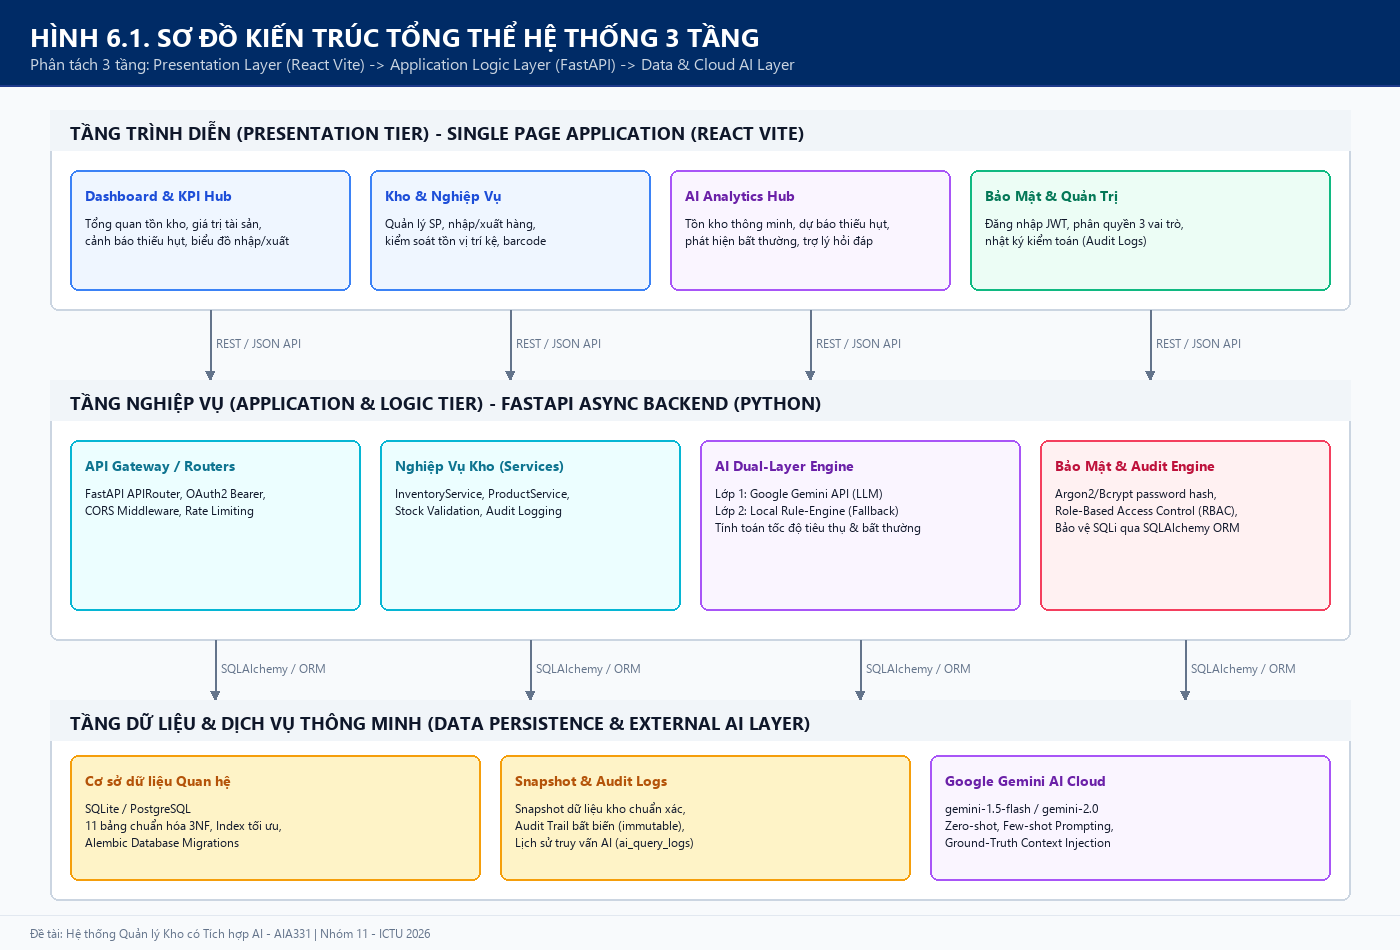
\includegraphics[width=0.92\textwidth]{figures/architecture.png}
\caption{Sơ đồ kiến trúc 3-Tier Client-Server của hệ thống quản lý kho tích hợp AI}
\end{figure}

\section{Sơ đồ luồng dữ liệu (Data Flow Diagram - DFD)}

Sơ đồ luồng dữ liệu mô tả trực quan cách thức dữ liệu di chuyển qua các tiến trình xử lý từ các tác tử người dùng vào các kho lưu trữ dữ liệu (Data Stores).

Ở mức ngữ cảnh (DFD Mức 0), hệ thống nhận các luồng dữ liệu đầu vào như thông tin đăng nhập, yêu cầu tạo phiếu nhập/xuất, câu hỏi tự nhiên từ người dùng; sau đó xử lý và trả về mã xác thực, kết quả giao dịch kho, các chỉ số KPI thời gian thực và báo cáo phân tích thông minh.

Ở mức phân rã chi tiết (DFD Mức 1), các tiến trình được chia tách thành: (1.0) Xác thực và phân quyền; (2.0) Quản lý danh mục \& nhà cung cấp; (3.0) Xử lý giao dịch Nhập kho; (4.0) Xử lý giao dịch Xuất kho chống âm; (5.0) Phân tích dữ liệu và Trợ lý AI.

Sơ đồ luồng dữ liệu DFD tổng hợp được trình bày tại Hình 6.2.

\begin{figure}[h!]
\centering
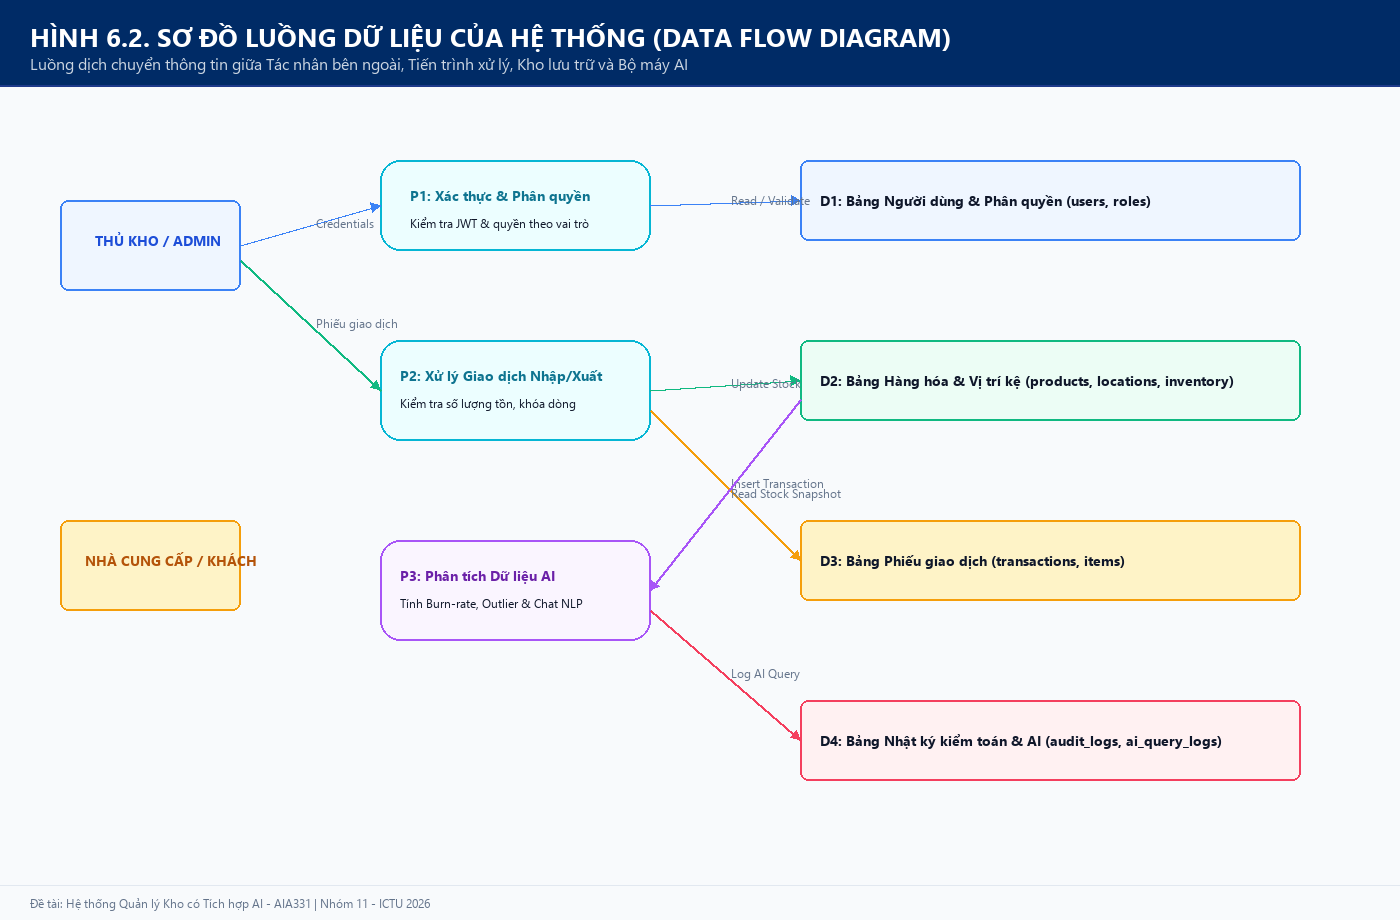
\includegraphics[width=0.92\textwidth]{figures/data_flow.png}
\caption{Sơ đồ luồng dữ liệu (DFD) Mức 0 và Mức 1 của hệ thống}
\end{figure}

